\documentclass[11pt,a4paper]{article}
\usepackage[utf8]{inputenc}
\usepackage{graphicx}
\usepackage{lscape}
\usepackage{pgfgantt}
\graphicspath{ {images/}}
\begin{document}
\thispagestyle{empty}
\begin{figure}
\centering
\begin{minipage}{.5\textwidth}
  \centering
  
\includegraphics[width=.7\linewidth]{hwlogo}
  \label{fig:test1}
\end{minipage}%
\begin{minipage}{.5\textwidth}
  \centering
  
\includegraphics[width=\linewidth]{roboticslogo}
  \label{fig:test2}
\end{minipage}
\end{figure}
{
\centering
\vspace{10mm}
{\huge Evolving a Learning Agent using Neuroevolution in the FightingICE Game Framework}\\
\vspace{20mm}
{\large Deliverable 1: Final Year Dissertation}\\
{\large Heriot-Watt University}\\
\vspace{10mm}
{\large Robert John Dunn\\
H00163867\\
BSc Honours in Computer Science\\
}
\vspace{10mm}
{\large Supervisor:}\\
Dr Patricia A. Vargas\\
School of Mathematical \& Computer Sciences\\
Heriot-Watt University
\vspace{3mm}\\
{\large Co-Supervisor:}\\
Dr Fabrício Olivetti de França\\
Center of Mathematics, Computing and Cognition\\
Federal University of ABC, Sao Paulo, Brazil
\vspace{3mm}\\
Second Reader:\\
Dr Mohamed Abdelshafy\\
School of Mathematical \& Computer Sciences\\
Heriot-Watt University\\}
\newpage
\thispagestyle{empty}
\vspace*{30mm}
\section*{Declaration}
I,  Robert Dunn confirm that this work submitted for assessment is my own and is expressed
in my own words. Any uses made within it of the works of other authors in any
form (e.g., ideas, equations, figures, text, tables, programs) are properly acknowledged
at any point of their use. A list of the references employed is included.\\

Signed: Robert John Dunn\\

Date: 24/11/2016 
\newpage
\thispagestyle{empty}
\begin{abstract}
Neuroevolution is a popular technique for machine learning in which the topology and/or weights of an artificial neural network are adjusted by an evolutionary algorithm. The technique takes inspiration from the evolution of the biological nervous system and is a popular approach for reinforcement learning problems. One way to demonstrate the effectiveness of neuroevolution is through artificial intelligence in games. This project aims to implement a learning agent in the FightingICE platform, a two-dimensional Java fighting game organised and maintained by Ritsumeikan University, Kyoto. The agent is designed to evolve through neuroevolution to improve its performance in the game, eventually becoming competitive versus a human opponent. By implementing a neuroevolution method in a simplistic environment, we hope to evaluate the effectiveness of neuroevolution as a method of machine learning and explore the potential of our agent's performance.
\end{abstract}
\newpage
\thispagestyle{empty}
\tableofcontents
\newpage
\section{Introduction}
\subsection{Motivation}
The ability to learn is a fundamental attribute of intelligent behaviour \cite{michalski}, in which one acquires knowledge or skills through study, experience, or being taught. The field of machine-learning aims to imitate this learning attribute and apply it to machines in order to improve their performance at tasks without being explicity programmed.\\

Various methods of machine-learning exist which allow the agent (machine) to adapt itself in order to process new data. One of these methods is neuroevolution, which involves the weights and/or topology of an artificial neural network being adjusted by an evolutionary algorithm. The neuroevolution method is loosely based on the way the biological nervous system operates: with neurons communicating through axons, represented by nodes of the neural network with weighted connections. Neuroevolution has received huge popularity due to the fact that many artificial intelligence problems can be cast as optimisation problems, and since the method is ground in biological metaphor and evolutionary theory. \cite{risi}\\

One way to test the effectiveness of machine-learning methods is through artificial intelligence in computer games. Since the state of a game is usually easily determined (e.g. the hit-points of both player's characters), the effectiveness of the learning method when controlling the agent's actions can be easily evaluated. The FightingICE platform \cite{fightingice}, is a two-dimensional fighting game written in Java by a group in Ritsumeikan University, Kyoto. The platform allows programming of artificially intelligent agents within the game and sends the agent delayed information about the current state of the game. 
\newpage
\subsection{Objectives}
This project aims to implement a neuroevolution algorithm acting on a learning agent in the FightingICE game platform. The inputs to the algorithm will be based on the agent's environment, such as the enemy's current position and the enemy's energy level, the outputs will be character actions e.g. move left, move right, attack. In order to increase the rate of the agent's evolution, an environment using incremental evolution will be used, exposing the agent to progressively more difficult challenges.\\

Once implemented, we will evaluate the algorithms performance versus a human opponent. We will use human volunteers of varying skill levels in the game, and record their performance versus the agent at different stages of its evolution. We will also compare the effectiveness of the algorithm to that of previous prototypes to evaluate any improvements made.\\

From this project, we hope to assess the effectiveness of neuroevolution as a method of machine-learning and gain the programming experience from implementing it. We also hope to find the potential to which an agent employing a neuroevolution method to learn can perform. Through comparisons of the algorithm to previous prototypes, we can also assess the progress of our algorithm over time and how improvements affect the agent's performance.
\newpage
\subsection{Professional, Legal, Ethical and Social Issues}
\subsubsection{Professional Issues}
A professional mindset will be employed when approaching this project. The mindset will involve appropriate communication with staff on the project and meeting deadlines reliably. Drafts will also be provided to the project supervisor with suitable time to provide feedback. When dealing with human participants for the agent testing, care will be taken to anonymise the participants data and ensure the data is protected accordingly.

\subsubsection{Legal Issues}
In order to avoid any legal issues during the project, we will ensure that any code or external work used is correctly referenced and the work holds an appropriate sharing license. This should prevent any copyright claims from outside sources. Since the project is a dissertation project for Heriot-Watt University and is purely for research purposes, there is not likely to be any legal issues arising.

\subsubsection{Ethical and Social Issues}
The majority of this project will be completed within a controlled, software-development environment, where ethical and social issues are of no concern. When human participants are involved for the agent evaluation, care will be taken to keep the environment safe and risk-free. Since only the use of a computer is involved for the evaluation, there are few potential risks.
\newpage
\section{Literature Review}
In this section of the dissertation, we will present any fundamental concepts used in the project. We will also discuss and evaluate relevant work in the field.
\subsection{Machine Learning}
Learning is a fundamental human function in which we modify our behaviour tendency according to experiences or teaching \cite{michalski}, to become better when a similar situation occurs. In the study of machine-learning, algorithms, computer applications, and systems, utilise learning to improve their performance at certain tasks. There are two main entities in the machine-learning model, the teacher and the learner. The teacher, while not always available, contains the knowledge to perform a given task while the learner has to learn the knowledge the teacher holds. \cite{swarmann} There are three types of machine learning:
\begin{itemize}
\item \emph{Supervised Learning}\\
A teacher provides the learner with a set of input and desired output pairs. The learner can then use these examples to improve its performance at the task.
\item \emph{Unsupervised/Self-organised Learning}\\
There is no teacher, so the learner learns based only on the observed relationships. A common application is finding patterns or grouping within data, using methods such as cluster analysis.
\item \emph{Reinforcement Learning}\\
The agent uses goal-directed learning where a notion of reward is introduced and the agent attempts to maximise this reward. There is no teacher for the agent and no explicit model of the environment. Computational approach to learning from interaction. \cite{reinforce}
\end{itemize}
\newpage
Another way to categorise machine-learning methods is by the output of the method. The output of the method is usually a good indication of the application of the method, for example, two classes of outputs 'spam' and 'not spam' in spam filtering. 
\begin{itemize}
\item \emph{Classification}\\
Inputs are assigned to two or more classes (groups) of output. Typically used with a supervised learning method. One application is spam filtering.
\item \emph{Regression}\\
Supervised learning problem similar to classification, however the outputs are continuous rather than discrete.
\item \emph{Clustering}\\
A set of inputs to be divided into groups. Unlike classification, groups are not defined beforehand. Typically an unsupervised learning task.
\item \emph{Density Estimation}\\
Finds the distribution of inputs in some space.
\item \emph{Dimensionality Reduction}\\
Inputs mapped into a lower-dimensional space.\\
\end{itemize}
Machine-learning is being applied extensively in modern day life, though not everyone is aware of it. The personalisation of search engine results and social networking feeds are one application, providing user's with appropriate content. \cite{search} Other examples of machine-learning application include optical character recognition (OCR) and computer vision. \cite{ocr}
\newpage
\subsection{Neuroevolution}
\subsubsection{Fundamentals}
Neuroevolution is a biologically-inspired method of machine learning in which an artificial neural network is evolved using an evolutionary algorithm. The biological inspiration for the method comes from the nervous system in which neurons communicate through axons, translated to machine-learning by the nodes of a neural network communicating through weighted connections.\\

The method has proved popular, especially in the fields of artificial life, evolutionary robotics and computer games. One reason for its popularity is the fact that neuroevolution is a form of reinforcement learning, which can be applied more generally than its counterpart, supervised learning. The popularity also stems from the fact that the method is ground in biological metaphor and evolutionary theory. The method consistently performs well in many areas of application and can handle large action/state spaces. \cite{risi}\\

The applications of neuroevolution are numerous and diverse. One application is the implementation of artificially intelligent agents in computer games (see section 2.2.5). Other applications include dynamic resource allocation, optimising manufacturing processes and even creating musical melodies. \cite{neapps}
\begin{figure}[h]
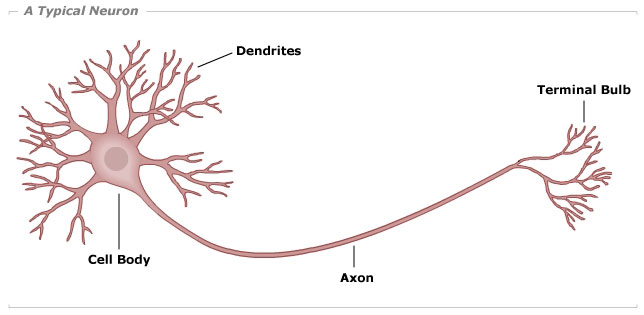
\includegraphics[width=\textwidth]{neuron}
\caption{Simple diagram of a biological neuron.}
\end{figure}
\newpage
\subsubsection{Artificial Neural Networks}
Artificial neural networks model the way the brain solves problems with collections of neurons communicating through axons, represented with nodes of the network with weighted connections. \\

The most basic version of an ANN (artificial neural network) is a perceptron. A perceptron is a simple machine which takes a variable number of input nodes which connect to a single output node. \cite{percept} The concept of the perceptron was extended by means of the the multi-layer feed forward network, which incorporates extra 'hidden' layers of nodes between the input and output. The more hidden layers there are, and the more nodes in these layers, the more complex behaviour a network can experience. \cite{ffann}\\

Neural networks can be employed in a variety of ways, for both supervised and unsupervised/reinforcement learning problems. Networks can have an associative (content-addressable) memory and can also implement parallel processing across individual nodes. \cite{nnm} Common applications for neural networks include character recognition, image compression and stock market prediction. \cite{nnapps}
\begin{figure}[h]
\centering{
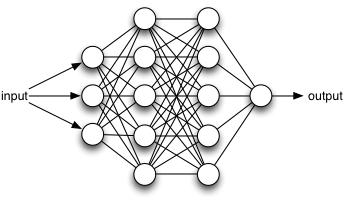
\includegraphics[width=0.8\textwidth]{ann}
\caption{Multi-layer feed forward network with labelled layers.}
}
\end{figure}
\newpage
\subsubsection*{Activation Function}
In order to calculate the output of a certain node in a network given the input or set or inputs, we use an activation function. \cite{activate} This output of the node is usually saturated to a value between minus and positive one by the function and then scaled appropriately when output. \cite{swarmann} \\

The simplest activation function is the step function \cite{nnm}, where if the weighted sum of the inputs to the node falls below a certain threshold the output is zero, else the output is one. This can be thought as the node either sending signals or not sending signals. The step function is used in perceptrons and often shows up in other models. \cite{percept} Since there are only two possible outputs of nodes using the step function, it is common to use different, more general functions.\\

One of these more general, non-linear activation function is the hyperbolic tangent function tanh, shown in figure 3. This allows nodes to have an activation output of a real number between negative one and one. The usage of these more general functions allows us to exhibit more complex behaviour within the network.
\begin{figure}[h]
\centering{
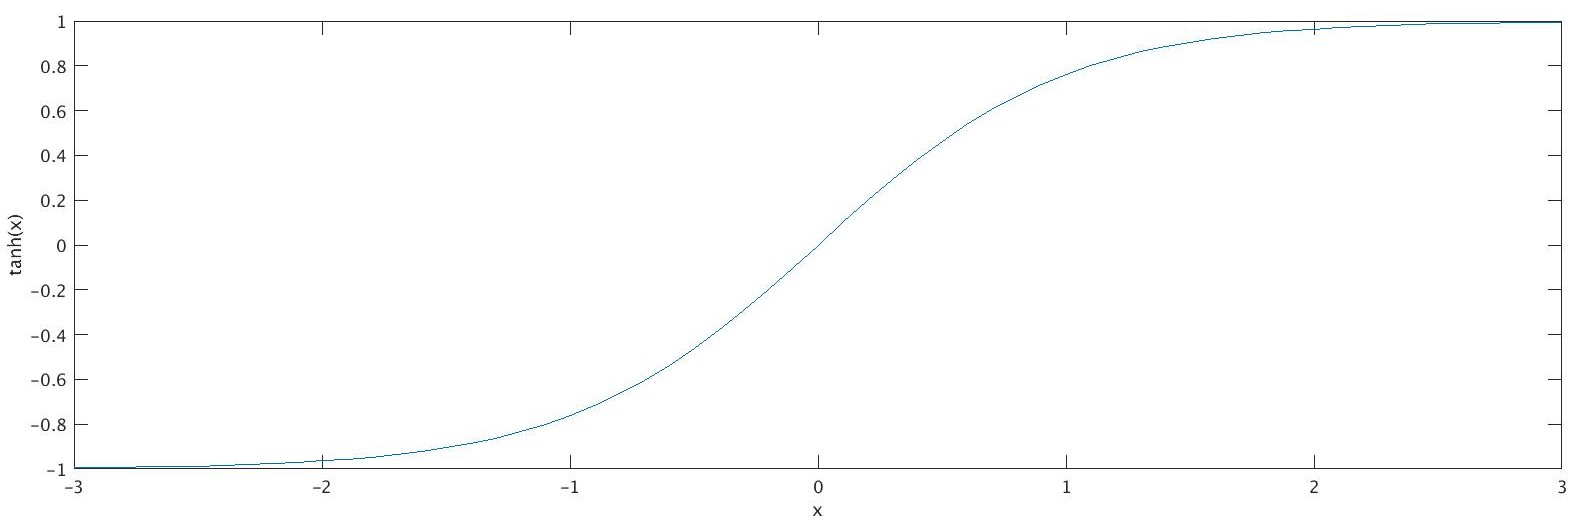
\includegraphics[width=0.8\textwidth]{tanh}
\caption{tanh activation function plot.}
}
\end{figure}
\newpage
\subsubsection{Evolutionary Algorithms}
Evolutionary algorithms are methods of optimisation, where potential solutions to the problem are seen as individuals of some population. Each individual in the population is assigned a fitness value which is calculated according to the performance of the provided solution, and the algorithm works to find the best (fittest) of these solutions. Using techniques inspired by biological evolution such as reproduction, mutation, recombination, and selection, new populations of solutions can be generated and assessed. Using evolutionary algorithms allows fine tuning of the search space through constants such as rate of reproduction and mutation rate. \cite{gas}\\

The implementation of an evolutionary method involves three steps which are repeated indefinitely \cite{ea}:
\begin{enumerate}
\item Generate population of initially random individuals.
\item Evaluate the fitness of each individual in the population.
\item Update and replace population with methods such as crossover and mutation.
\end{enumerate}
\newpage
\subsubsection{Incremental Evolution}
When an agent is provided with a complex behaviour, it may have trouble evolving to perform at its potential. Using incremental evolution, the behaviour can be learnt incrementally with tasks gradually increasing in difficulty. This form of evolution proved effective in at least one implementation \cite{incre}. The agent's task was a prey capture task: the agent moves through the environment and must catch its prey before the set number of time-steps. With increasingly difficult tasks, the agent was able to rapidly improve its performance, and skip many potential generations of evolution.\\

We hope to experiment with the usage of incremental evolution in our project to assess whether it has a positive impact on the evolution of the agent.\vspace{10mm}
\subsubsection{NEAT (NeuroEvolution of Augmenting Topologies)}
NeuroEvolution of Augmenting Topologies (NEAT) is a method of neuroevolution developed by Ken Stanley in 2002, which involves both the weights and the topology of the ANN being altered. The method is a genetic algorithm and involves applying the following three techniques: \cite{neat}
\begin{enumerate}
\item Track genes with history markers to allow crossover among topologies
\item Apply speciation to preserve innovations
\item Developing topologies incrementally from simple initial structures
\end{enumerate}
A notable extension of NEAT which could potentially be appropriate for the project is HyperNEAT. HyperNEAT is a hypercube-based extension of the method developed by the Evolutionary Complexity Research Group at UCF. \cite{hypehype} \cite{hyperneat}
\newpage
\subsection{FightingICE}
\subsubsection{Game Platform}
FightingICE is a Java based game platform organised and maintained by Intelligent Computer Entertainment Lab., Ritsumeikan University. The game is based in an arena where two fighters are competing versus each other, attempting to deplete the other's hit-points while preserving their own. The FightingICE platform was designed to allow easy development and evaluation of artificially agents in the game for research or hobby purposes. Once implemented, an agent receives information about the state of the game from the platform periodically, such as the opponent player's location and current energy levels. A delay is added to this game information in order to simulate the delay a human player would experience from reaction time. \cite{fightingice}\\

\subsubsection{Game Agents}
There are four characters available in the game: Zen, Garnet, Lud, and Kfm. Each of the characters is capable of moving, performing attacks, and combining these attacks into unique combos. The game starts with each player at 0 hit-points and 0 energy. Once a player successfully connects an attack against its opponent, the player's energy is increased and the opponent's hit-points decrease. In order to compete against an opponent, the character must dodge opposing attacks and make effective use of energy to land attacks and reduce the opponent's hit-points.\\
\begin{figure}[h]
\centering{
\includegraphics[width=\textwidth]{fightingICE}
\caption{Screenshot of the FightingICE platform in action.}
}
\end{figure}
\newpage
\subsection{Related Work}
When implementing neuroevolution, a computer game is a common choice of environment. Neuroevolution methods have been used as artificial intelligence in games in the following external projects:
\begin{itemize}
\item Improving AI for simulated cars. \cite{pace}
\item Neuroevolution approach to general video game playing. \cite{genvid}
\item Calculating optimal jungling routes in the game DOTA2. \cite{dota}
\item Using neuroevolution to play atari games. \cite{atari}
\end{itemize} 
The work has found neuroevolution to be an effective machine-learning algorithm in a computer game environment and the method proved to operate consistently across a diverse range of games.\\

There are also numerous agents programmed in the FightingICE platform to compete in competitions. \cite{fightingice} We will test and assess the performance of a select few agents at a later stage of this project. Hopefully from this assessment of the agents we can evaluate the strategies of the programmer to improve the agent's performance as well as the effectiveness of different methods of AI.

\newpage
\section{Organisation}
In this section we present the decision process on how to approach the task including analysis of the task itself, analysis of the requirements, and analysis of the risks. A gantt chart of the project timeline is also included.
\subsection{Project Task Analysis}
The objective of this project is to evolve an agent in the FightingICE game platform with a neuroevolution method. The agent will be evolved to the point of being competitive versus a human opponent. \\

In order to implement the neuroevolution method, we will first need an artificial neural network to control the actions of the agent. The neural network will need to take as input various factors from its environments such as the location of the opposing player, the energy of the opposing player and whether the opponent is performing an attack. The outputs of the neural network will be actions for the character, for example move left, jump, attack. Once a neural network controlling the agent has been implemented, the network must be evolved to imitate the learning process. This will involve deciding on a suitable evolutionary algorithm and the encoding of the network's genotype. It will also need to be decided whether only the weights of the network are evolved, or also augmenting the topology (NEAT) and/or altering the activation function.\\

To improve the rate of evolution for the agent, we will create an incremental evolution environment where the agent is exposed to tasks of gradually increasingly difficulty. To implement this environment, we will limit the capabilities of the training opponent and gradually return them.\\

To test whether the agent's performance has improved to the point of being competitive versus a human opponent, we will find volunteers of varying skills to face our agent in the game. The results of the player versus our agent at various stages of its evolution can then be evaluated to assess the effectiveness of the neuroevolution algorithm which we implemented.
\newpage
\subsection{Requirement Analysis}
\subsubsection{Table of Requirements}
\begin{tabular}{|p{0.1\linewidth}|p{0.5\linewidth}|p{0.1\linewidth}|p{0.2\linewidth}|}
\hline
No. & Requirement & Priority & Predecessors\\ \hline
1 & Implement a neural network to control agent's behaviour & High &\\ \hline
1.1 & Initialise a network with random weights, test if the sensors can be read and the actions can be output & High &\\ \hline
1.2 & Implement a simple rule-based agent for the agent to compete versus & High & 1.1\\ \hline
1.3 & Test and execute at least one agent from the FightingICE AI competition & Medium &\\ \hline
2 & Implement an appropriate evolutionary algorithm to evolve the neural network & High & 1\\ \hline
2.1 & Test whether a simple evolutionary algorithm evolving the weights of the network improves the agent's performance & High & 1\\ \hline
2.2 & Adapt and use the HyperNEAT method, test whether it improves on the previous algorithm & Medium & 1, 2.1\\ \hline
3 & Create an incremental evolution environment for the agent & Medium & 1, 2\\ \hline
3.1 & Limit the capabilities of the opponent and incrementally return them to test whether speed of evolution is improved & Medium & 1, 2\\ \hline
3.2 & Evolve against a simple agent, replace opponent with best agent after convergence and continue & Medium & 1, 2\\ \hline 
4 & Evaluate the agent's performance versus a human opponent at various stages of its evolution & High & 1, 2\\ \hline
\end{tabular}
\newpage
\subsubsection{Requirements Textual Descriptions}
\subsubsection*{1 - Implement a neural network to control agent's behaviour}
To implement an agent in the FightingICE platform controlled by a simple neural network.
\subsubsection*{1.1 - Initialise network with random weights, test if sensors can be read and actions can be output}
In order to test whether sensors can be read and actions can be output, initialise a simple neural network with random weights to control the agent. Ensure game information is being received and number of outputs nodes match character actions.
\subsubsection*{1.2 - Implement a simple rule-based agent for the agent to compete versus}
Create agent in FightingICE which follows simple rule-based logic. Use as an opponent for the neuroevolution agent while it is evolving.
\subsubsection*{1.3 - Test and execute at least one agent from the FightingICE AI competition}
Find agents from the FightingICE AI Competition and test them to see strategies of other programmer's work. Attempt to read and understand the code.
\subsubsection*{2 - Implement an appropriate evolutionary algorithm to evolve the neural network}
Find and implement an appropriate evolutionary algorithm to evolve the ANN of the agent. Decide on implementation based on performance evaluation.
\subsubsection*{2.1 - Test whether a simple evolutionary algorithm evolving the weights of the network improves the agent's performance}
Implement a simple EA such as hill-climbing or an algorithm using only mutation to evolve the agent's neural network. Test whether the evolution improves the agent's performance and if so, to what extent.
\newpage
\subsubsection*{2.2 - Adapt and use the HyperNEAT method, test whether it improves on the previous algorithm}
Replace the previous evolutionary algorithm with an implementation of the HyperNEAT or other appropriate neuroevolution method. Test the new implementation versus the rule-based agent to test whether it improves on the previous algorithm.
\subsubsection*{3 - Create an incremental evolution environment for the agent}
Create an incremental evolution environment to speed the process of evolution for the agent.
\subsubsection*{3.1 - Limit the capabilities of the opponent and incrementally return them to test whether speed of evolution is improved}
Initially, completely limit the capabilities of the agent's opponent and gradually return these capabilities over time. Evaluate whether gradually exposing the agent to these capabilities improved the speed of evolution of the agent.
\subsubsection*{3.2 - Evolve against a simple agent, replace opponent with best agent after convergence and continue}
Begin evolution with simple rule-based opponent. Once convergence in evolution occurs, replace the agent's opponent with the current best agent. Repeat this process incrementally and compare performance of each opponent with that of its successors.
\subsubsection*{4 - Evaluate the agent's performance versus a human opponent at various stages of its evolution}
Test the performance of different agents at different stages of their evolution against human players. Attempt to find volunteers that rank at different skill levels from novice to expert. From this we can assess whether the agent was evolved to become competitive versus a human opponent.

\newpage
\subsection{Performance Assessment}
\subsubsection{Table of Project Prototypes}
\begin{tabular}{|p{0.4\linewidth}|p{0.2\linewidth}|p{0.4\linewidth}|}
\hline
Objective & Date & Assessment\\ \hline
Prototype 1: Agent using neural network to sense environment and output simple actions in FightingICE & 15/12/2016 & Agent can proficiently perceive its environment and output simple actions\\ \hline
Prototype 2: Agent controlled by neural network being evolved by simple evolutionary algorithm, altering only the weights of the network & 20/01/2017 & Evaluate agents performance versus simple AI opponent at different stages of its evolution\\ \hline
Prototype 3: Agent evolved with HyperNEAT or other appropriate neuroevolution method & 10/02/2017 & Evaluate agent's performance versus AI and compare whether method was more effective than simple EA\\ \hline
Prototype 4: Agent with appropriate learning method implemented in incremental evolution environment & 10/03/2017 & Agent's environment is adapted to utilise incremental evolution. Agent's performance assessed and compared versus learning without incremental environment.\\ \hline
\end{tabular}
\newpage
\subsubsection{Prototypes Textual Descriptions}
\subsubsection*{Prototype 1}
The initial prototype will involve an agent using an artificial neural network to test if the agent's environments can be sensed and the agent can output actions on the platform. Once we have evaluated the agent's functionality we will move towards evolving the neural network.

\subsubsection*{Prototype 2}
The second prototype will implement a simple evolutionary algorithm in order to alter the weights of the neural network. With an appropriate fitness function for the agent, this method of evolution should result in improvement of the agent's performance. The agent's performance versus both a simple rule-based opponent and a human opponent will be evaluated.

\subsubsection*{Prototype 3}
The third prototype for the project will involve implementing the HyperNEAT neuroevolution method for the agent. Should we find another, more appropriate, neuroevolution method to apply, we will take it into consideration. Once implemented, the agent utilising the HyperNEAT algorithm will be assessed versus both the rule-based and a human opponent.

\subsubsection*{Prototype 4}
The final prototype for the project will utilise incremental evolution techniques to improve its rate of evolution. This prototype is due to be finished by the 10th March 2017 and will mark the end of our agent development. Once the final prototype has been completed, evaluation of the agent's performance will commence.
\newpage
\subsection{Risk Assessment}
\subsubsection{Table of Risks}
\begin{tabular}{|p{0.1\linewidth}|p{0.4\linewidth}|p{0.2\linewidth}|p{0.3\linewidth}|}
\hline
No. & Risk Name & Probability & Response\\ \hline
1 & Laptop failure & Low & Online storage (github), backups\\ \hline
2 & Difficulties with Java programming & Low & Spend more time familiarising with language and practising\\ \hline
3 & Difficulties with FightingICE platform & Medium & Consult tutorials and relevant documentation from website\\ \hline
\end{tabular}
\subsubsection{Risks Textual Description}
\subsubsection*{1 - Laptop failure}
In the case of the laptop being used to develop the project failing, essential code or documentation could be lost. To reduce the impact of this risk, we will ensure to regularly upload the code to a online repository such as GitHUB. We will also back-up any work on external hard-drives or on the university computers.
\subsubsection*{2 - Difficulties with Java programming}
To avoid any problems with lack of Java programming expertise, we will spend time familiarising ourselves with the language before development.
\subsubsection*{3 - Difficulties with FightingICE platform}
Since there is plenty of information and lots of tutorials on agent development with the platform, we should be able to easily familiarise ourselves with it.
\newpage
\subsection{Project Plan}
Figure 5 shows a gantt chart representing a timeline for the completion of the project including all prototypes, the dissertation and the project poster. With this project plan we hope to leave appropriate time to evaluate any results as well as carefully thought out prototype deadline which will result in any code problems occurring early. The plan has been shown to and approved by both the project supervisor and co-supervisor.
\newpage
\begin{landscape}
{\centering
\subsubsection{Gantt Chart}
}
\vspace{10mm}
\begin{ganttchart}[vgrid, hgrid]{1}{24}
	\gantttitle{2016}{9}
	\gantttitle{2017}{15} \\
	\gantttitle{Oct}{3}
	\gantttitle{Nov}{3}
	\gantttitle{Dec}{3}
	\gantttitle{Jan}{3}
	\gantttitle{Feb}{3}
	\gantttitle{Mar}{3}
	\gantttitle{Apr}{3}
	\gantttitle{May}{3}
	\\
	\ganttbar{Deliverable One (03/10/2016 - 24/11/2016)}{1}{5}\\
	\ganttbar{Complete Interview (24/11/2016 - 16/12/2016)}{6}{11}\\
	\ganttgroup{Prototypes}{6}{17}\\
	\ganttbar{Prototype One (24/11/2016 - 15/12/2016)}{6}{8}\\
	\ganttlinkedbar{Prototype Two (16/12/2016 - 20/01/2017)}{9}{11}\\
	\ganttlinkedbar{Prototype Three (23/01/2017 - 13/02/2017)}{12}{13}\\
	\ganttlinkedbar{Prototype Four (14/02/2017 - 14/03/2017)}{14}{17}\\
	\ganttbar{Results Evaluation (15/03/2017 - 10/04/2017)}{18}{19}\\
	\ganttbar{Complete Dissertation (10/04/2017 - 24/04/2017)}{20}{20}\\
	\ganttbar{Project Poster (24/04/2017 - 19/05/2017)}{21}{23}\\
\end{ganttchart}	
\end{landscape}
\newpage
\section{Methodology and Results}
\subsection{Prototype One: Artificial Neural Network in Game Framework}
\subsubsection{Design}
The initial prototype of a simple ANN was implemented without the use of any Java libraries.
\subsubsection{Implementation}
The neural network is implemented in the class NeuralNetwork which provides methods to both initialise the network and feed through the network to determine output. When the class is initialised, a network is created with three input nodes, ten hidden and seven output. Weights for the network are stored as two arrays of doubles, each corresponding to a separate layer of the network and are initialised using a Java Random object to a value between minus one and one. Inputs are fed through the network with the feed() method which returns an array of doubles representing the activations of the output layer nodes. The method first calculates the activations of hidden layer nodes using the initial inputs and weights of the network, then using the hidden activations it is possible to calculate activations for the output.

In order to implement the network into the FightingICE game framework a controller class called Prototype1 was used. The class implements the AIInterface interface provided with FightingICE in order to read input and send output to the game. The inputs for the network are the X-coordinate of the agent, the Y-coordinate of the agent and the agent's energy, which are all provided with appropriate methods from he CommandCenter class. Before feeding the inputs into the network, they are normalised using the hyperbolic tangent function to have inputs within the range minus one to one. After being fed through the network, the output activations are used to determine which buttons will be pressed by the agent. 
\subsubsection{Evaluation}

\newpage
\subsection{Prototype Two: Weights of Neural Network Evolved by Genetic Algorithm}
\subsubsection{Design}
\subsubsection{Implementation}
\subsubsection{Evaluation}
\subsection{Prototype Three: Network Evolved using HyperNEAT Method}
\subsubsection{Design}
\subsubsection{Implementation}
\subsubsection{Evaluation}
\subsection{Prototype Four: Appropriate Learning Method Implemented in Incremental Evolution Environment}
\subsubsection{Design}
\subsubsection{Implementation}
\subsubsection{Evaluation}
\newpage
\section{Testing and Performance Assessment}
\section{Conclusions}
\newpage
\section{Appendices}
\subsection*{Figure 1}
Image of a biological neuron\\
https://online.science.psu.edu/sites/default/files/bisc004/content/neuron.jpg
\subsection*{Figure 2}
Image of a simple multi-layer feedforward artificial neural network.\\
 https://upload.wikimedia.org/wikipedia/commons/thumb/e/e4/Artificial\_ neural\_network.svg/2000px-Artificial\_neural\_network.svg.png
\subsection*{Figure 3}
Plot of the tanh activation function.\\
http://www.mpe.mpg.de/~ott/dpuser/tanh.png
\subsection*{Figure 4}
Screenshot of the FightingICE game platform.\\
https://i.ytimg.com/vi/\_Poz6qwIwbc/maxresdefault.jpg
\subsection*{Figure 5}
Gantt chart of the project timeline.\\
Created in GanttProject application.
\newpage
\section{References}
\begin{thebibliography}{10}

\bibitem{michalski}
	Michalski, R., Carbonell, J. and Mitchell, T.
	(1983).
	Machine Learning: An Artificial Intelligence Approach. 
	pp. 5-20.
	

\bibitem{nnm}
	Wilde, P.
	(1997).
	Neural Network Models.
	[book]
	pp. 4-14.
	
\bibitem{reinforce}
	Barto, S. and Sutton R.
	(1998).
	Reinforcement Learning: An Introduction.
	pp. 23-30.
	
\bibitem{search}
	McCallum, A., Nigam, K., Rennie, J. and Seymore, K.
	(2001).
	A Machine Learning Approach to Building Domain-Specific Search Engines.
	[online]
	Available at: http://www.kamalnigam.com/papers/cora-ijcai99.pdf
	[Accessed 23 Nov. 2016]
	
\bibitem{ocr}
	Wernick, M., Yang, Y. and Strother, S.
	(2010).
	Machine Learning in Medical Imaging.
	[online]
	Available at: https://www.ncbi.nlm.nih.gov/pmc/articles/PMC4220564/
	[Accessed 23 Nov. 2016]
	
\bibitem{ea}
	Prins, C.
	(2004).
	A simple and effective evolutionary algorithm for the vehicle routing problem.
	[book]
	pp. 20-35.	

\bibitem{neapps}
	Neural Networks Research Group
	(2014).
	Research on Neuroevolution Applications.
	[online]
	Available at: http://www.cs.utexas.edu/users/nn/pages/research/ne-applications.html
	[Accessed 23 Nov. 2016]
	
\bibitem{fightingice}
	Intelligent Computer Entertainment Lab, Ritsumeikan University.
	(2010).
	FightingGameAICompetition.
	[online]
	Available at: http://www.ice.ci.ritsumei.ac.jp/~ftgaic/
	[Accessed 23 Nov. 2016]

\bibitem{risi}
	Risi, S. and Togelius, J.
	(2015).
	Neuroevolution in Games: State of the Art and Open Challenges.
  	[online]
  	Available at: https://arxiv.org/pdf/1410.7326.pdf
  	[Accessed 03 Nov. 2016]

\bibitem{pace}
	Pace, A.
	(2014).
	Improving AI for simulated cars using Neuroevolution.
	[online]
	Available at: http://commerce3.derby.ac.uk/ojs/index.php/gb/article/view/3/1
	[Accessed 07 Nov. 2016]
	
\bibitem{lampro}
	Lampropoulos, A.
	(2005).
	Machine Learning Paradigms.
	[online]
	Available at: http://file.allitebooks.com/20150722/Machine\%20Learning\%20Para-digms-\%20Applications\%20in\%20Recommender\%20Systems.pdf
	[Accessed 18 Nov. 2016]
  
\bibitem{incre}
	Gomez, F. and Miikkulainen, R.
	(1997).
	Incremental Evolution of Complex General Behaviour
	[online]
	Available at: http://nn.cs.utexas.edu/downloads/papers/gomez.adaptive-behavior.pdf
	[Accessed 18 Nov. 2016]
	
\bibitem{dota}
	Batsford, T.
	(2014).
	Calculating Optimal Jungling Routes in DOTA2 Using Neural Networks and Genetic Algorithms.
	[online]
	Available at: http://commerce3.derby.ac.uk/ojs/index.php/gb/article/view/14/12
	[Accessed 18 Nov. 2016]
	
\bibitem{atari}
	Hausknecht, M., Lehman, J. and Stone, P.
	(2014).
	A Neuroevolution Approach to General Atari Game Playing.
	[online]
	Available at: https://www.cs.utexas.edu/~mhauskn/papers/atari.pdf
	[Accessed 15 Nov. 2016]
	
\bibitem{genvid}
	Braylan, A., Hollenbeck, M., Meyerson, E. and Miikkulainen, R.
	(2015).
	Reuse of Neural Modules for General Video Game Playing
	[online]
	Available at: https://arxiv.org/pdf/1512.01537v1.pdf
	[Accessed 17 Nov. 2016]
	
\bibitem{swarmann}
	Dehuri, S., Ghosh, S., and Cho, S-B
	(2011).
	Integration of Swarm Intelligence and Artificial Neural Network.
	[book]
	P1-P23

\bibitem{percept}
	Widrow, B. and Lehr, A.
	(1990).
	30 Years of Adaptive Neural Networks: Perceptron, Madaline, and Backpropagation.
	[online]
	Available at: https://pdfs.semanticscholar.org/8b73/adda1-5fa71b0a35ffedb899d6a72d621923b.pdf
	[Accessed 24 Nov. 2016]
	
\bibitem{ffann}
	Hornik, K.
	(1989).
	Multilayer Feedforward Networks are Universal Approximators.
	[online]
	Available at: http://deeplearning.cs.cmu.edu/pdfs/Kornick\_et\_al.pdf
	[Accessed 24 Nov. 2016]
	
\bibitem{nnapps}
	Stanford University.
	(2013).
	Applications of neural networks.
	[online]
	Available at: http://cs.stanford.edu/people/eroberts/courses/soco/projects/neural-networks/Applications/index.html
	[Accessed 24 Nov. 2016]
	
\bibitem{activate}
	Hornik, K.
	(1990).
	Approximation Capabilities of Multilayer Feedforward Networks.
	[online]
	Available at: http://zmjones.com/static/statistical-learning/hornik-nn-1991.pdf
	[Accessed 24 Nov. 2016]
	
\bibitem{gas}
	Vavak, F. and Fogarty, T.
	(1996).
	Comparison of Steady State and Generational Genetic Algorithms for Use in Nonstationary Environments.
	[online]
	Available at: http://citeseerx.ist.psu.edu/viewdoc/download?doi=10.1.1.55.3585-\&rep=rep1\&type=pdf
	[Accessed 24 Nov. 2016]
	
\bibitem{neat}
	Kenneth, S. and Miikkulainen, R.
	(2002).
	Evolving neural networks through augmenting topologies.
	[book]
	pp. 1-30.
	
\bibitem{hyperneat}
	Kenneth, S., D'Ambrosio, D. and Gauci, J.
	(2009).
	A hypercube-based encoding for evolving large-scale neural networks.
	[book]
	pp. 05-09.
	
\bibitem{hypehype}
	Evolutionary Complexity Research Group at UCF.
	(2003).
	The hypercube-based neuroevolution of augmenting topologies (HyperNEAT).
	[online]
	Available at: http://eplex.cs.ucf.edu/hyperNEATpage/
	[Accessed 24 Nov. 2016]
\end{thebibliography}
\end{document}